\documentclass[11pt, a4paper]{article}
\usepackage[utf8]{inputenc}
\usepackage[margin=.7in]{geometry}
\usepackage{listings}
\usepackage{setspace}
\usepackage{xcolor}
\usepackage{titlesec}
\usepackage{enumitem}
\usepackage{amssymb}
\usepackage{amsmath}
\usepackage{bm}
\usepackage{multicol}
\usepackage{graphicx}
\graphicspath{{./Figures/}}
\usepackage{color}
\usepackage{hyperref}
\hypersetup{
	colorlinks=true,
	linkcolor=blue,
	urlcolor=blue,
}
\titleformat*{\section}{\LARGE\bfseries\filcenter}
\titleformat*{\subsection}{\Large\bfseries}
\titleformat*{\subsubsection}{\large\bfseries}
\definecolor{codegreen}{rgb}{0,0.5,0}
\definecolor{codegray}{rgb}{0.5,0.5,0.5}
\definecolor{codered}{rgb}{0.78,0,0}
\definecolor{codepurple}{rgb}{0.58,0,0.68}
\definecolor{backcolour}{rgb}{0.95,0.95,0.92}
\lstdefinestyle{Pythonstyle}{
	language = Python,
    backgroundcolor=\color{backcolour},   
    commentstyle=\color{gray},
    keywordstyle=\color{codegreen},
    numberstyle=\tiny\color{codegray},
    stringstyle=\color{codered},
    basicstyle=\ttfamily\footnotesize,
    breakatwhitespace=false,         
    breaklines=true,                 
    captionpos=b,                    
    keepspaces=true,                 
    numbers=left,                    
    numbersep=5pt,                  
    showspaces=false,                
    showstringspaces=false,
    showtabs=false,                  
    tabsize=2,
    morekeywords = {as},
    keywordstyle = \color{codegreen}
}
\lstset{style=Pythonstyle}

\begin{document}
	\begin{titlepage}
		\begin{center} \Huge \textbf{Udacity: Intro to ML with PyTorch} \end{center}
		\tableofcontents
		\newpage
	\end{titlepage}
%%%% PAGE 1 %%%%

	\begin{spacing}{1.1}
	\section{Supervised Learning}
	\subsection{Linear Regression}
	\textbf{Absolute Trick}: A point at $(p,q)$ with a line $y = w_1x + w_2$, we want to change the line to slowly move it towards the point. We want to do this by a small value $\alpha$ (learning rate), so our line become $\hat{y} = (w_1 + p\alpha)x + (w_2 + \alpha)$. \vspace*{2mm}\\
	\textbf{Square Trick}: Similar to the absolute trick, but we consider the offset of the point from the y-axis ($p$) and from the line ($q-q'$) where $q'$ is the \textit{estimated} $y$ point and $q$ is the actual $y$ point. So our line becomes $\hat{y} = (w_1 + p(q-q')\alpha)x + (w_2 + (q-q')\alpha)$\vspace*{2mm}\\
	\textbf{Mean Absolute Error}: the average of the sum of the distance between the estimate line value $\hat{y}$ and actual $y$ value, giving us the equation: $Error = \frac{1}{m} \sum_{i=1}^{m}|y-\hat{y}|$ \vspace*{2mm}\\
	\textbf{Mean Squared Error}: Similar to MAE, but we square the value instead which gives us a square near the value $y-\hat{y}$. This gives us the equation: $Error = \frac{1}{2m} \sum_{i=1}^{m}(y-\hat{y})^2$ \vspace*{2mm}\\
	\textbf{Gradient Step}: $w_i \rightarrow w_i - \alpha\frac{\partial}{\partial w_i}Error$ with $\frac{\partial}{\partial w_1}Error = -(y-\hat{y})x$ and $\frac{\partial}{\partial w_2}Error = -(y-\hat{y})$
	\begin{lstlisting}
	X : array of predictor features
	y : array of outcome values
	W : predictor feature coefficients
	b : regression function intercept
	learn_rate : learning rate
	
	yhat = np.matmul(X,W) + b # predicted values
	error = y-yhat
	W_new = W + learn_rate*np.matmul(error,X) # updated slope
	b_new = b + learn_rate*error.sum() # updated y-intercept \end{lstlisting}\vspace*{3mm}
	\textbf{Higher Dimensions}: $\hat{y} = w_1x_1 + w_2x_2 + ... + w_{n-1}x_{n-1} + w_n$ \vspace*{2mm}\\
	\textbf{Polynomial Regression}: Allows us to add degrees to our $x$ to better find our line.
	\begin{lstlisting}
	import numpy as np
	import pandas as pd
	from sklearn.preprocessing import PolynomialFeatures
	from sklearn.linear_model import LinearRegression
	
	train_data = pd.read_csv('data.csv')
	X = np.asarray(train_data['Var_X']).reshape((20,1))
	y = np.asarray(train_data['Var_Y']).reshape((20,1))
	
	poly_feat = PolynomialFeatures(degree=4) # 4th degree polynomial
	X_poly = poly_feat.fit_transform(X)
	
	poly_model = LinearRegression(fit_intercept=False).fit(X_poly, y) \end{lstlisting}\vspace*{3mm}
	\textbf{L1 Regularization}: adds the absolute value of the coefficients ($w_i$) to the error. This is computationally inefficient, better when data is sparse, gives us feature selection (makes irrelevant columns to 0). \vspace*{2mm}\\
	\textbf{L2 Regularization}: we add the square of the coefficients ($w_i$) to the error. This is computationally efficient, better for non-sparse data, doesn't have feature selection (treats all columns equally).  \vspace*{2mm}\\
	\textbf{$\mathbb{\lambda}$ Parameter}: determines how much impact the coefficients have on our total error. Choosing a large $\lambda$ leads to simpler models more while a small $\lambda$ leads to more complex models. \newpage
%%%% PAGE 2 %%%%

	\noindent We can train a Linear Regression model with L1 regularization applied to it by using the \href{https://scikit-learn.org/stable/modules/generated/sklearn.linear_model.Lasso.html}{Lasso model}.
	\begin{lstlisting}
	import pandas as pd
	from sklearn.linear_model import Lasso
	
	train_data = pd.read_csv('data.csv', header=None)
	X = train_data.iloc[:,:-1] # all rows, all colums up to last
	y = train_data.iloc[:,-1] # all rows, last column
	
	lasso_reg = Lasso().fit(X, y)
	
	reg_coef = lasso_reg.coef_
	print(reg_coef)
	# [ 0.  2.35793224  2.00441646 -0.05511954 -3.92808318  0.]	\end{lstlisting}\vspace*{3mm}
	\textbf{Feature Scaling}: a way of transforming your data into a common range of values (2 ways below).\vspace*{2mm}\\
	\textbf{Standardizing}: turning the column into a standard normal variable by computing $\frac{x-\mu}{\sigma}$ and is interpreted as the number of standard deviations each value is away from the mean (most common type).\vspace*{2mm}\\
	\textbf{Normalizing}: data is scaled between 0 and 1 by calculating $\frac{x-x.min}{x.max - x.min}$\vspace*{2mm}\\
	\textbf{Distance Based Metrics}: If an algorithm uses distance based metrics to predict, choosing some sort of feature scaling is necessary (such as for SVMs of k-nn).\vspace*{2mm}\\
	\textbf{When using Regularization}: we need all columns to have equal ranges so they are treated similar when calculating the penalty. We need features with small ranges and large ranges to have similar coefficients.
	\begin{lstlisting}
	import pandas as pd
	from sklearn.preprocessing import StandardScaler
	from sklearn.linear_model import Lasso
	
	train_data = pd.read_csv('data.csv', header=None)
	X = train_data.iloc[:, :-1]
	y = train_data.iloc[:, -1]
	
	scaler = StandardScaler()
	X_scaled = scaler.fit_transform(X)
	
	
	lasso_reg = Lasso().fit(X_scaled, y)
	
	reg_coef = lasso_reg.coef_
	print(reg_coef)
	# [0.   3.90753617   9.02575748  -0.   -11.78303187   0.45340137]	\end{lstlisting}\vspace*{3mm}
	Notice how after we scaled the features, the L1 regularization set the 1st and 4th columns coefficients to zero. Where when we did not standardize in the previous code, the L1 regularization set the 1st and 6th columns coefficients to zero. \newpage
%%%% PAGE 3 %%%%

	\subsection{Perceptron Algorithm}
	\textbf{Linear Boundaries}: we use a boundary line to determine how to classify the data, denoted by the equation $w_1x_1 + w_2x_2 + b = 0$ which we rewrite as $Wx+b = 0$ where $W=(w_1,w_2)$ and $x=(x_1,x_2)$. Note that we just take the dot product of $W\cdot x \implies w_1x_1 + w_2x_2$. We then classify the output of the boundary line by:
	$$\hat{y} = \begin{cases}
	1 \text{ if } Wx+b \geq 0\\
	0 \text{ if } Wx+b < 0
	\end{cases} $$
	\textbf{Higher Dimensions}: if we are working with $n$ columns, our boundary line becomes a $n-1$ dimensional hyperplane with the equation $w_1x_1 + w_2x_2 + ... + w_nx_n + b = 0 \implies Wx+b = 0$. The prediction works the same way as the linear boundary. Note that weights (W) is a (1xn) row vector, input (x) is a (nx1) column vector, and bias (b) is a (1x1) vector.\vspace*{2mm}\\
	\textbf{Basic Perceptrons}: We have our input nodes ($x_1,...,x_n$ and can also include our bias $b$) which are then multiplied by the corresponding weights ($w_1,...,w_n$), which are then inputted into a linear function node ($Wx+b$), and finally that input is sent to a step function node (determines if $\hat{y}$ is 1 or 0).\vspace*{2mm}\\
	\textbf{Updating the line}: In a 2D example, with point $(p,q)$, we can update the boundary line with the equation $ (w_1\pm\alpha p)x_1 + (w_2\pm\alpha q)x_2 + (b\pm\alpha*1)$. Note that $\pm$ depends on which way we move the line.
	\begin{lstlisting}
	def perceptronStep(X, y, W, b, learn_rate = 0.01):
		for i in range(len(X)): # go through all points
			yhat = prediction(X[i], W, b) # get predicted values
			if y[i] - yhat == 1: # if y=1 but yhat=0 (move line down)
				W[0] += learn_rate*X[i][0]
				W[1] += learn_rate*X[i][1]
				b +=learn_rate
			if y[i] - yhat == -1: # if y=0 but yhat=1 (move line up)
				W[0] -= learn_rate*X[i][0]
				W[1] -= learn_rate*X[i][1]
				b -=learn_rate    
		return W, b	\end{lstlisting} \vspace*{2mm}
	
	\subsection{Decision Trees}
	\textbf{(Multiclass) Entropy}: $-\sum_{i=1}^np_i log_2(p_i)$ where $p_i$ is the probability for each class. Note that points with the same color will have zero entropy, so this is the ideal outcome for classification. \vspace*{2mm}\\
	\textbf{Information Gain}: Tells us how well our data is being classified (in a range between 0 and 1). The lower the information gain, the worse our model is doing as separating the data. The higher the information gain, the better our model is performing at classification. We have the formula: \\$IG = Entropy(Parent) - \Big[\frac{m}{m+n}Entropy(Child_1)+\frac{n}{m+n}Entropy(Child_2)\Big]$ \vspace*{2mm}\\
	\textbf{Important Hyperparameters for Decision Trees}: \vspace*{1mm} \\
	\textbf{Maximum depth}: the largest possible length between the root to a leaf, a tree of maximum length $k$ can have at most $2^k$ leaves. \vspace*{2mm}\\
	\textbf{Minimum samples to split}: numeric value ($m$) that says if a node doesn't have at least $m$ samples it can't split.\vspace*{2mm}\\
	\textbf{Minimum samples per leaf}: decides how many samples must be in each node. If it is an integer, then it is a sample size. If it is a float, it is a percentage of samples needed in a leaf. \vspace*{2mm}\\
	\textbf{WARNING}: Large depth often causes overfitting. Small depth can result in a very simple model, which may cause underfitting. Small minimum samples per split may result in overfitting. Large minimum samples may result in the tree not having enough flexibility to get built, and may result in underfitting. \newpage
%%%% PAGE 4 %%%%

	\begin{lstlisting}
	import pandas as pd
	import numpy as np
	from sklearn.model_selection import train_test_split
	from sklearn.tree import DecisionTreeClassifier
	from sklearn.metrics import accuracy_score
	import random
	random.seed(42)
	
	in_file = 'titanic_data.csv'
	full_data = pd.read_csv(in_file)
	
	outcomes = full_data['Survived'] # Labels
	features_raw = full_data.drop('Survived', axis = 1) # Remove label from features df
	
	features_no_names = features_raw.drop(['Name'], axis=1) # Remove names
	
	features = pd.get_dummies(features_no_names) # One-hot encoding
	features = features.fillna(0.0)
	
	len(features.columns) # 839
	# Note that we now have 839 columns instead of 11 since each ticket is a column
	# from the one-hot encoding (each ticket_number is now a column with all 0's 
	# expect for the person/row with the ticket, which will be a 1).
	
	X_train, X_test, y_train, y_test = train_test_split(features, outcomes, 
	                                                    test_size=0.2, random_state=42)
	
	model = DecisionTreeClassifier().fit(X_train, y_train)
	
	# Making predictions
	y_train_pred = model.predict(X_train)
	y_test_pred = model.predict(X_test)
	train_accuracy = accuracy_score(y_train, y_train_pred) # 1.0
	test_accuracy = accuracy_score(y_test, y_test_pred) # 0.8156
	# High training and lower test accuracy means we might be overfitting.
	
	# Tune the hyperparameters for new model to improve test score
	model_tune = DecisionTreeClassifier(max_depth=20, min_samples_leaf=6)
	model_tune.fit(X_train, y_train)
	tune_y_train_pred = model_tune.predict(X_train)
	tune_y_test_pred = model_tune.predict(X_test)
	tune_train_accuracy = accuracy_score(y_train, tune_y_train_pred)
	tune_test_accuracy = accuracy_score(y_test, tune_y_test_pred) 
	
	print('Train Acc: {}, Test Acc: {}'.format(tune_train_accuracy, tune_test_accuracy))
	# Train Acc: 0.8820224719101124, Test Acc: 0.8603351955307262 \end{lstlisting} \newpage
%%%% PAGE 5 %%%%

	\subsection{Naive Bayes}
	\textbf{Naive Bayes}: a supervised machine learning algorithm that can be trained to classify data into multi-class categories. The probabilistic model computes the conditional probabilities of the input features and assigns the probability distributions to each of possible classes. \vspace*{2mm}\\
	\textbf{Bayes Theorem}: We have prior probabilities for a given problem, and after we know that event $B$ occurred, we can find the posterior probability with the formula $ P(A_j|B) = \frac{P(B|A_j)P(A_j)}{\sum P(B|A_i)P(A_i)}$\vspace*{2mm}\\
	\textbf{Naive Assumption}: $P(A\cap B) = P(A)P(B)$ meaning that the two events are independent. We assume this to be true even if it is not the case. \vspace*{2mm}\\
	\textbf{Conditional Probability (Proportional)}: $P(A|B_1,B_2,...,B_n) \propto P(B_1,B_2,...,B_n|A)P(A)$\vspace*{2mm}\\
	\textbf{Algorithm}: For an event A, we have $ P(A|B_1,B_2,...,B_n) \propto \frac{P(B_1|A)P(B_2|A)...P(B_n|A)P(A)}{P(B_1,B_2,...,B_n)}$  \vspace*{2mm}\\
	\textbf{Bag of Words (BoW)}: a collection of text data where we count the frequency of the words. \vspace*{2mm}\\
	\textbf{Accuracy}: the ratio of the number of correct predictions to the total number of predictions.\vspace*{2mm}\\
	\textbf{Precision}: a ratio of true positives to all positives (true+false positive).\vspace*{2mm}\\
	\textbf{Recall (Sensitivity)}: a ratio of true positives to all the words (true positives + false negatives).\vspace*{2mm}\\
	\textbf{F1 Score}:  is the weighted average of the precision and recall scores (between 0 and 1, higher better).
	\begin{lstlisting}
	import pandas as pd
	from sklearn.model_selection import train_test_split
	from sklearn.feature_extraction.text import CountVectorizer
	from sklearn.naive_bayes import MultinomialNB
	from sklearn.metrics import accuracy_score, precision_score, recall_score, f1_score
	
	# Read in data from table, add column names, specify seperator
	df = pd.read_table('smsspamcollection/SMSSpamCollection', sep='\t', 
	                   names=['label', 'sms_message'])
	
	# Convert labels to numerical encodings
	df['label'] = df.label.map({'ham':0, 'spam':1})
	
	X_train, X_test, y_train, y_test = train_test_split(df['sms_message'], df['label'], 
                                                      random_state=1)
	
	count_vector = CountVectorizer()
	# Note that CountVectorizer automatically converts to lowercase and ignores
	# all punctuation. We can add stop_words=English if we want to ignore
	# common english words (a, an, and) in our matrix.
	
	# Fit the training data and return the frequency matrix
	training_data = count_vector.fit_transform(X_train)
	
	# Transform testing data and return the matrix (don't fit testing data)
	testing_data = count_vector.transform(X_test)
	
	naive_bayes = MultinomialNB()
	naive_bayes.fit(training_data, y_train)
	predictions = naive_bayes.predict(testing_data)
	
	print('Accuracy score: ', format(accuracy_score(y_test, predictions))) # 0.98851
	print('Precision score: ', format(precision_score(y_test, predictions))) # 0.972067
	print('Recall score: ', format(recall_score(y_test, predictions))) # 0.94054
	print('F1 score: ', format(f1_score(y_test, predictions))) # 0.95604 \end{lstlisting} \newpage
%%%% PAGE 6 %%%%

	\subsection{Support Vector Machines (SVMs)}
	\textbf{Classification Error}: we have a line separating our data points into groups, $Wx+b = 0$, and we want to add two more lines called the \textit{margin}. The line above has equation $Wx+b = 1$ and the line below has equation $Wx+b = -1$. We then assign points error based on where they are in respect to the margin:
	\begin{center}
	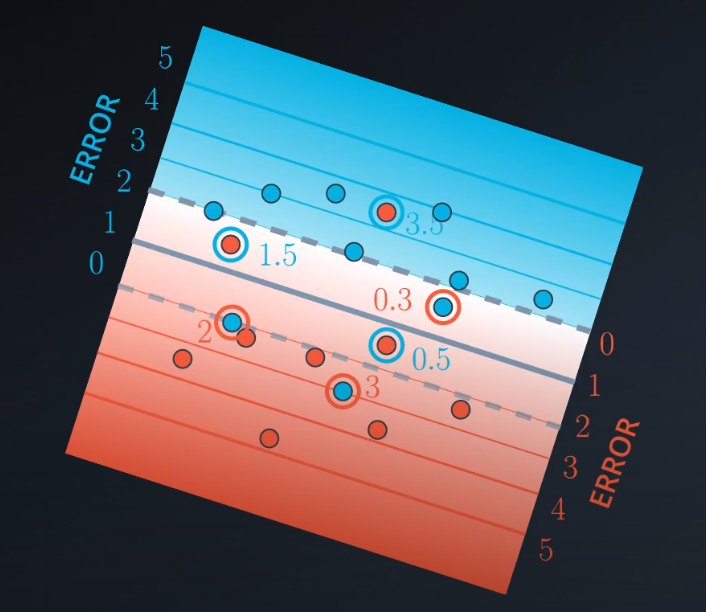
\includegraphics[scale=.3]{SVM}
	\end{center}
	\textbf{Classification Error}: we take the absolute value of all misclassified points and add them together. \vspace*{2mm}\\
	\textbf{Margin}: we want a small error if the margin is large, and a large error if the margin is small. We can determine the size of the margin by $\frac{2}{|W|}$ (2 divided by the norm of $W$). \vspace*{2mm}\\
	\textbf{Margin Error}: $|W|^2$ (note this is the same value given by L2 regularization). \vspace*{2mm}\\
	\textbf{Error Function}: we want Error = Classification Error + Margin Error, which we will minimize using gradient descent. \vspace*{2mm}\\
	\textbf{The C Parameter}: Error = C*Classification Error + Margin Error. It is a constant we use to determine the influence of the classification error. Large C means focus on classifying points (smaller margin), small C means focus on margin error (makes more classification errors).\vspace*{2mm}\\
	\textbf{Linear Kernel}: we separate our data using a linear line (doesn't work well when data is complicated).\vspace*{2mm}\\
	\textbf{Polynomial Kernel}: we separate our data using circles, hyperbolas, parabolas, and many more boundaries by adding more dimensions to our data to classify it. The degree of the polynomial determines what kind of boundaries we can create.\vspace*{.5mm}\\
	ex: (degree 2) $\mathbb{E}^2 \rightarrow \mathbb{E}^5: (x,y) \rightarrow(x,y,x^2,xy,y^2)$. We map our points (x,y) to a higher dimensions which allows us to create degree 2 functions. We then find a boundary hyperplane and map this back to a 2nd degree polynomial boundary (think of a paraboloid in 3D mapping back to a circle in 2D). \vspace*{2mm}\\
	
	
	
	
	
	
	
	
	
\end{spacing}
\end{document}